\section{\huge{Bonusopgaver}}

\setlength{\parindent}{3mm}

\subsection{Opgave 0}

Din IP-instruktor har fået besked på at lave en sjov SML-opgave, men han har
ikke lært at formulere sig letforståeligt, så du får følgende:

Skriv en SML-funktion \texttt{multifilter} med typen \texttt{($\alpha$ -> bool)
  list -> $\alpha$ list -> $\alpha$ list}.  Funktionen tager en liste af
funktioner og en liste af $\alpha$-værdier, og giver den liste tilbage, hvor det
for hvert element \texttt{x} i listen gælder at \texttt{x} er en del af
inddatalisten af $\alpha$-værdier, og at \texttt{f(x) = true} for hver funktion
\texttt{f} i listen af funktioner, og at uddatalisten har samme sortering som
inddatalisten.

Du må kun bruge funktioner fra \texttt{List}-modulet.


\subsection{Opgave 1}

Din vens mor vil lave en opgave om grafer, men hun kan ikke finde på nogen
analogi, og desuden er hun ikke særlig god til at tegne grafer.

Brug Prims algoritme til at finde det mindst udspændte træ for grafen:
\begin{center}
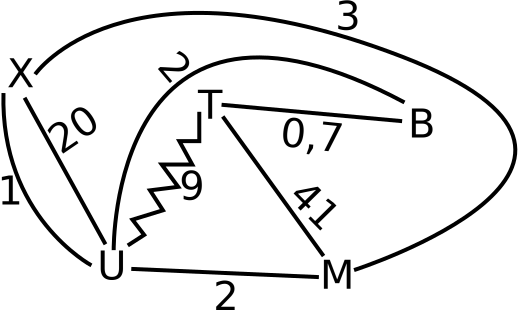
\includegraphics[width=.8\textwidth]{figures/graf.pdf}
\end{center}


\newpage
\subsection{Opgave 2}

I det følgende program har funktionen \texttt{f} dynamisk virkefelt der virker
over funktionsgrænser, mens funktionen \texttt{g} har statisk virkefelt.

\begin{verbatim}
int x = 10;                int g(int z) {
                             return f(z - x);
int f(int y) {             }
  return x + y;
}                          int run() {
                             int x = 3;
                             return g(1);
                           }
\end{verbatim}

\noindent{}Hvad returnerer \texttt{run()}?


\subsection{Opgave 3}

For at undgå flaskehalse har Kantinebestyrelsen anskaffet sig en ny colaautomat
med et flerbrugersystem, så nu kan $n > 1$ brugere købe cola fra den samme
automat samtidigt.  Automaten blev leveret med følgende enterprise-kode:
\begin{verbatim}
int antal_colaer = 1000;

void køb_en_cola() {
  afspil_fanfare();
  if (antal_colaer > 0) {
    træk_kroner(14);
    antal_colaer--;
    giv_cola();
  }
}
\end{verbatim}
Antag at koden køres samtidigt af flere brugere.  Lokalisér kapløbsstriden og
reparér den med en lås.


\subsection{Opgave 4}

Giv et formelt bevis for at
\begin{align*}
\forall x P(x) \lor \forall x Q(x) \lor \forall x R(x) \Rightarrow
\forall x \left(P(x) \lor Q(x) \lor R(x)\right)
\end{align*}


\subsection{Exercise 5}

This one's also for our international guests!

Half-Broken Car in Heavy Traffic (or ``HBCHT'') is a programming language for
the modern, dystopic age.  You define a two-dimensional grid in which you place
road redirections, a car, and an exit.  You then let the car follow the road
redirections.  Unfortunately, the car is half-broken and can never turn left,
relative to its current heading.

A program must contain exactly one car and exactly one exit.  When a program
starts, the car turns to a random direction -- either south, west, north, or
east.  After the initial car heading has been determined, the car moves one step
in that direction, determines its new direction, moves one step in that
direction, and so on, until it maybe reaches the exit.  If the car is at
position $(x, y)$, moving north puts it at $(x, y - 1)$, south at $(x, y + 1)$,
west at $(x - 1, y)$, and east at $(x + 1, y)$.  Moves ``wrap around'', so that
e.g. $(0, y)$ moved west becomes $(x_{max}, y)$, where $x_{max}$ is the highest
$x$ value.

The basic road redirections are ``go east'', ``go west'', ``go north'', and ``go
south''.  If the car moves to a position where there is a redirection, the car
changes heading unless that means turning left (relative to its current
heading).

To use the car for computations, a scheme has been set up whereby road
redirections double as instructions in a minimal tape-based instruction set.
The program uses a memory tape with cell IDs from $-\infty$ to $+\infty$, and a
program starts on cell $0$.  All cells have the initial value $0$ and contain
arbitrary precision integers.  The following table describes the road
redirection semantics, along with a final road redirection, and the shorthands
used for programming a grid.

{
\scriptsize
\begin{center}
\begin{tabular}{l|c|p{4cm}}
Redirection & Shorthand & Tape semantics\\\hline
Car start position & \texttt{o} & -\\
Highway exit & \texttt{\#} & Halt program\\
Go east & \texttt{>} & Increment memory cell pointer\\
Go west & \texttt{<} & Decrement memory cell pointer\\
Go north & \textasciicircum & Increment current memory cell value\\
Go south & \texttt{v} & Decrement current memory cell value\\
Maybe go east & \texttt{/} & Go east if the current memory cell $n$ has the same value as
cell $n - 1$; else continue
\end{tabular}
\end{center}
}

\noindent\textbf{6 (a)} Write a program in HBCHT that increments cell 0 and
exits, without causing any other lasting effects, i.e. all other cell values
must have the value $0$ (the start value) when the car hits the exit.

\noindent\textbf{6 (b)} Prove or disprove that HBCHT is Turing complete.


\subsection{Opgave 6}

$k$ dataloger står på den samme linje på en cirkulær løbebane med omkreds på 1
meter.  Startskuddet går, og de begynder alle samtidigt at løbe.  Hver datalog
har en unik løbehastighed.

En fysiker opstiller en konjektur: For alle $k \geq 0$ gælder at der for hver af
de $k$ dataloger findes et tidspunkt hvor datalogen er mindst $\frac{1}{k}$ m
væk fra enhver anden datalog i cirklen.

Bevis eller modbevis konjekturen.

\vspace{.1in} \textbf{\emph{NB: Der udloddes en flaske snaps til den første som
    kommer op i baren med en korrekt besvarelse af denne opgave!}}

% Uløst problem: Lonely runner conjecture

\setlength{\parindent}{0mm}
